\chapter{Measurements}
\label{chap:measurement}

In order to be able to validate the results obtained from the latter finite element simulation, specific measurements have been carried out. In this chapter, the acoustic power measurement of sound source and the outer pressure field measurement around carbody are presented. The obtained sound power spectral of the omnidirectional loudspeaker provide simulation input for the finite element analysis in section \ref{section:boundary_conditions}. Furthermore, the measurement results of outer pressure field serve as validation for the finite element model in chapter \ref{chap:results}.

\section{Characterisation of sound source}

Two important characteristics of a sound source are directivity and sound power. For the validation measurement, a dodecahedron loudspeaker of type Brüel \& Kjaer 4292-L is used as excitation, which can be treated as an omnidirectional sound source. Hence, only the sound power emmited by the loudspeaker is of interest. In the following, the acoustic power spectrum of the sound source is measured following ISO 9614-2 \cite{din19969614}.

\subsection*{Measurement setup}

In fig. \ref{fig:soundpowersetup} the measurement setup for the determination of sound power levels is shown. The omnidirectional loudspeaker is placed on a concrete reflective floor and is enveloped by a 1m x 1m x 1m reference box. The loudspeaker is driven by a reference amplifier with pink noise as input signal (fig. \ref{fig:signalgenerator}). In order to reduce flactuation in output power, the amplifier is switched on and warmed up for at least 20 minutes before the start of the measurement.

The measurement is carried out according to the ISO 9614-2 standard, in which the sound power is determined from intensity measurement over measruement surfaces. This method has the advantage that room reflections and any sound sources outside of the
reference box do not influence the measurment result.

The intensity measurements are done using the Brüel \& Kjaer sound intensity probe kit type 3654, which includes a pair of microphones that are placed face
to face to each other, seperated by a spacer. That is why this method of intensity measurement is also called two-microphone method or $p-p$ method. Instead of
direct measurement, the particle velocity is obtained by a finite-difference approximation to the pressure gradient. \cite{jocobsen_2005}\cite{moschioni_2008}

From the euler equation of motion
\begin{equation}
    \rho_0 \frac{\partial \Vec{u}}{\partial t} = -\nabla p \approx -\frac{p_2 - p_1}{\Delta r}
\end{equation}
where $p_1$ and $p_2$ are the measured pressure of the microphone closer and further from the incident sound wave, respectively and $\Delta r$ the thickness of the spacer.

Hence, the particle velocity can be calculated from the two pressures
\begin{equation}
    \Vec{u} = \int\frac{(p_1 - p_2)}{\rho \Delta r}\partial t
\end{equation}

The instantaneous sound intensity is obtained by the product of the approximated particle velocity and mean of the two measured pressures
\begin{equation}
    \Vec{I} = p\Vec{u} = \frac{p_1 + p_2}{2} \int\frac{(p_1 - p_2)}{\rho \Delta r}\partial t
\end{equation}

Fig. \ref{fig:scanningmethod} shows the intensity measurement using scan method. For the scanning, the intensity probe is moved over the surface with a constant speed and is kept perpendicular to the scanned area so that only the normal component of intensity is captured:
\begin{equation}
    I_n = \Vec{I} \cdot \Vec{n}
\end{equation}
where $\Vec{n}$ is the unit normal vector of the measurement surface. Each partial measurement surface is scanned twice, using vertical and horizotal scan path, respectively. The obtained result is the spatial-averaged intensity. The sound power of a single measurment surface is given by the product of the spatial average intensity and the surface area:
\begin{equation}
    P_i = \langle I_{ni}\rangle S_i
\end{equation}

The total sound power of the enclosed sound source is given by:
\begin{equation}
    P_{total} = \sum_{i = 1}^{N} P_i
\end{equation}

% Beispiel für eine Grafik
\begin{figure}[H]
\begin{center}
\includegraphics[width=12cm]{fig/Sound_power_measurement.png}
\caption{Setup for sound power measurement}
\label{fig:soundpowersetup}
\end{center}
\end{figure}

\begin{figure}[H]
     \centering
     \begin{subfigure}[b]{0.5\textwidth}
         \centering
         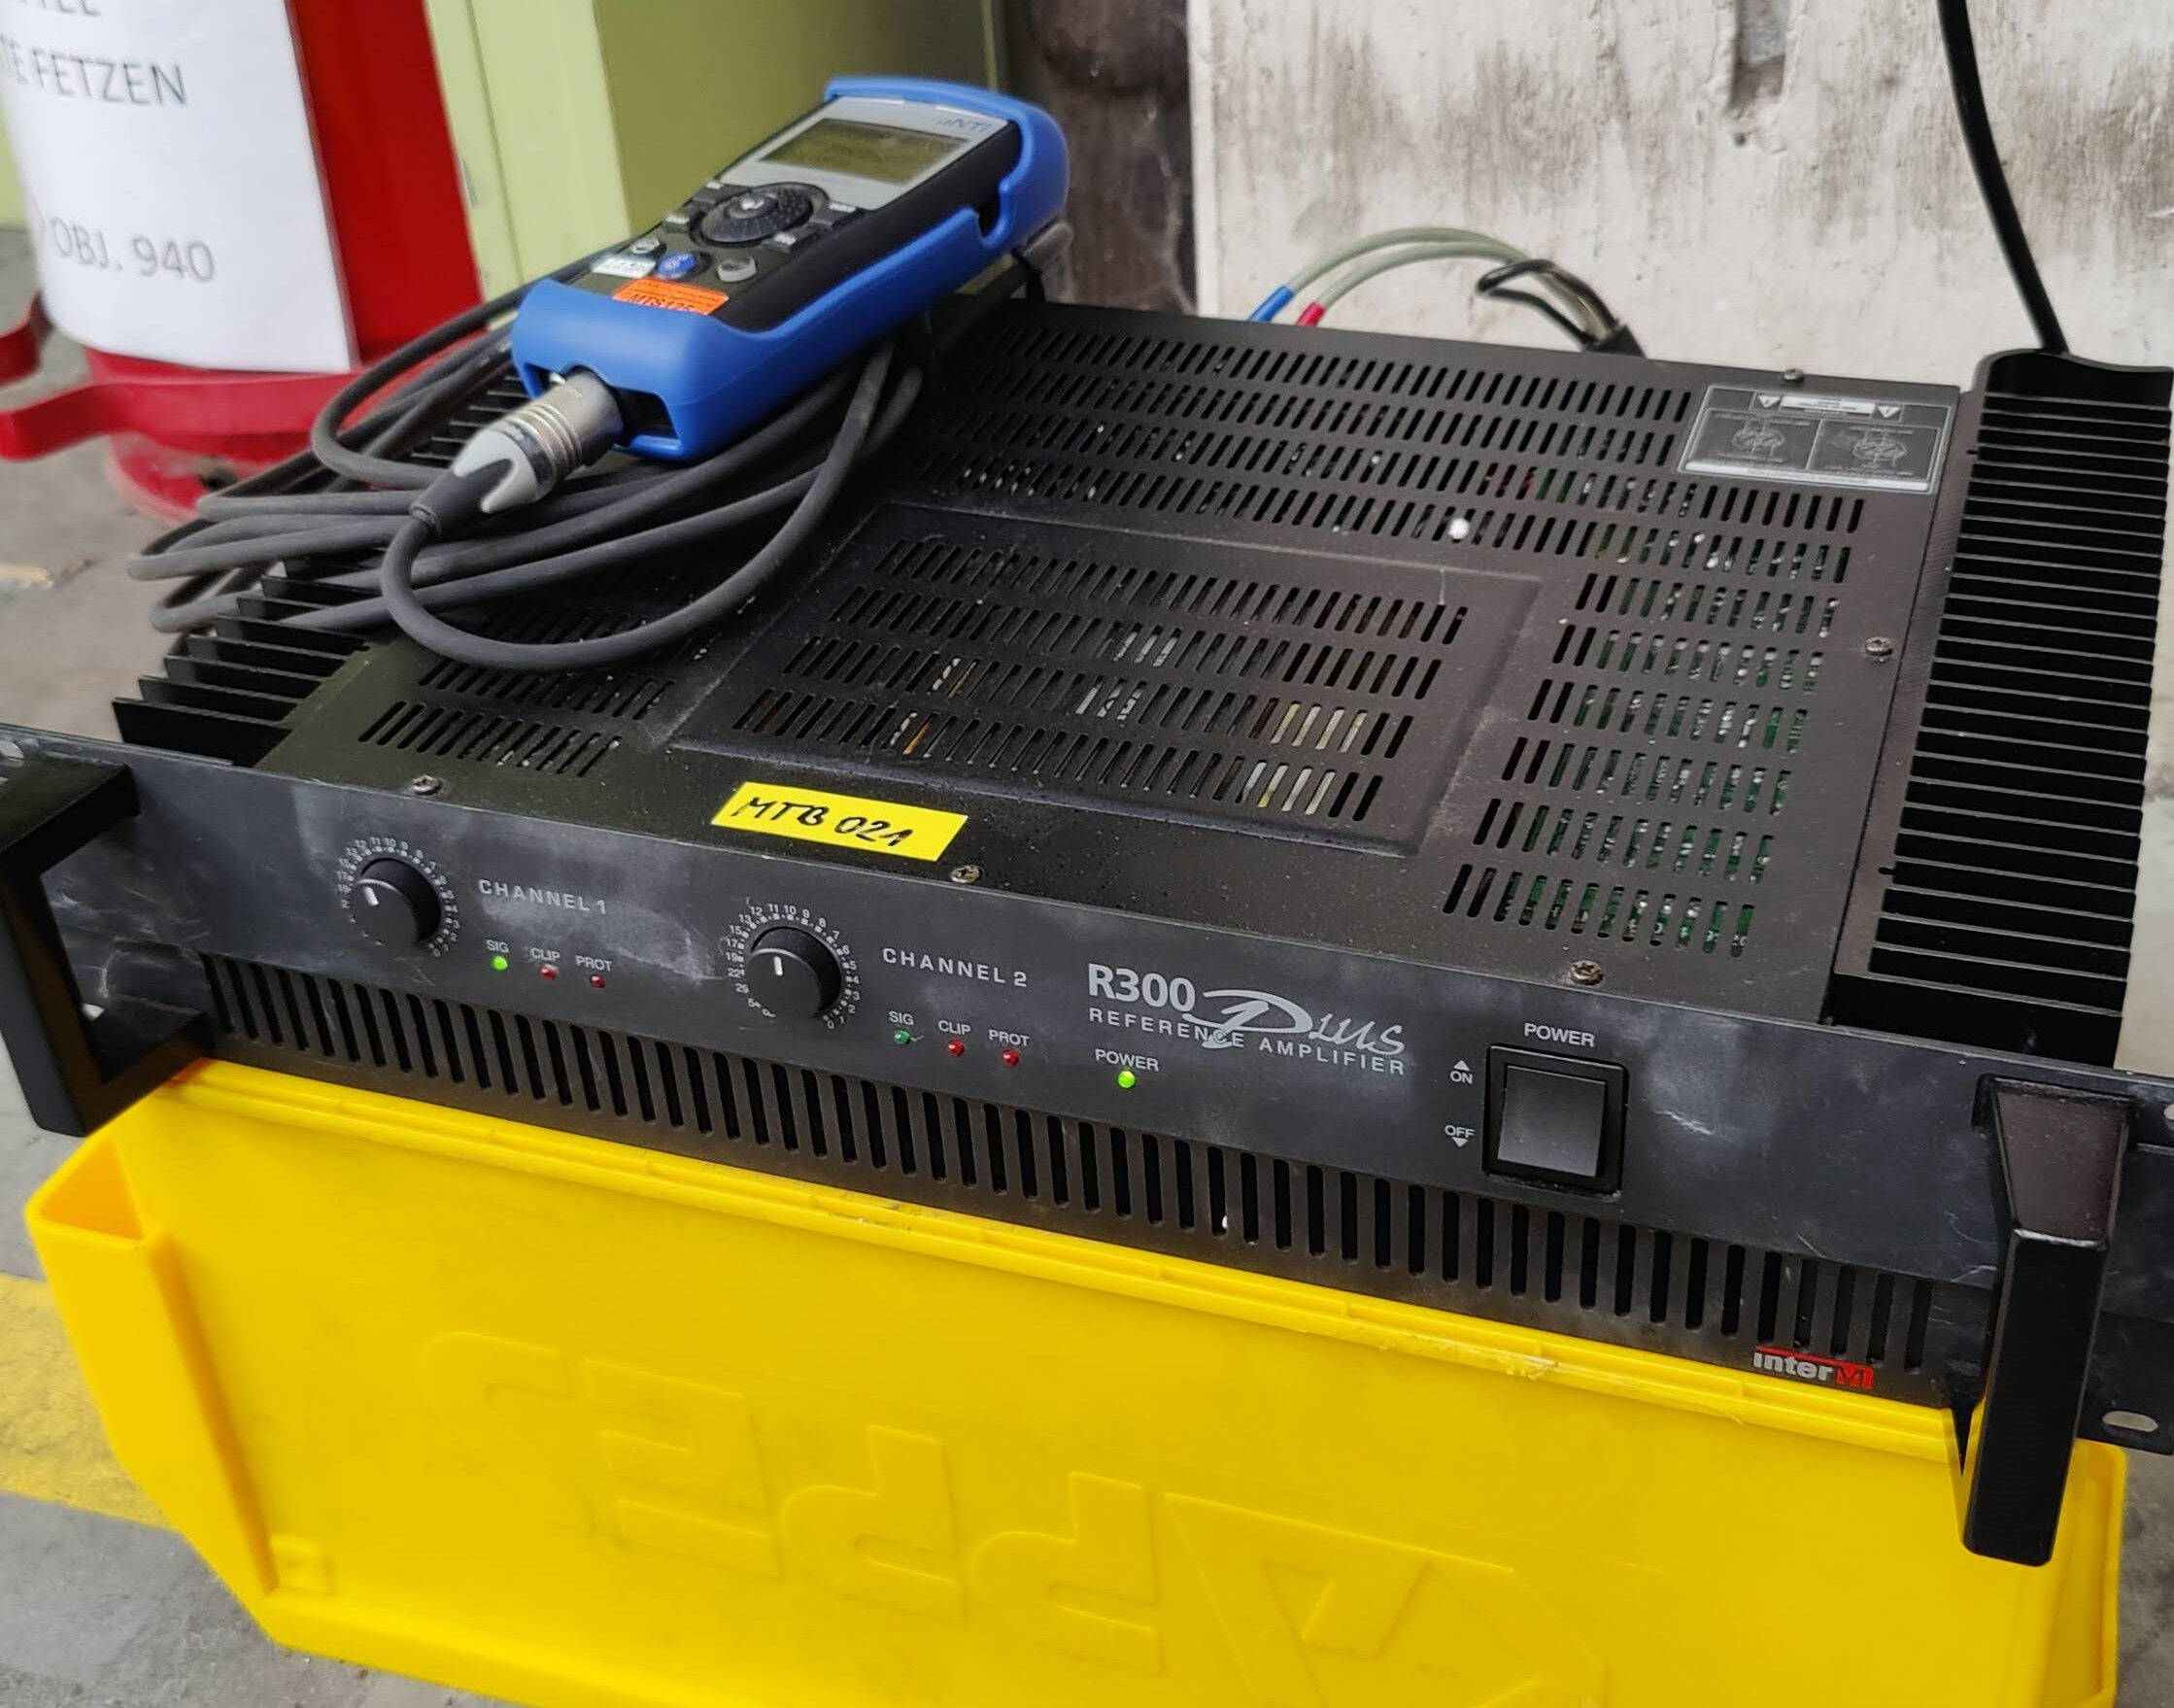
\includegraphics[width=\textwidth]{fig/amplifier_and_signal_generator.jpg}
         \caption{Inter-M R300 Plus reference amplifier}
     \end{subfigure}
     \hspace{0.1\textwidth}
     %\hfill
     \begin{subfigure}[b]{0.3\textwidth}
         \centering
         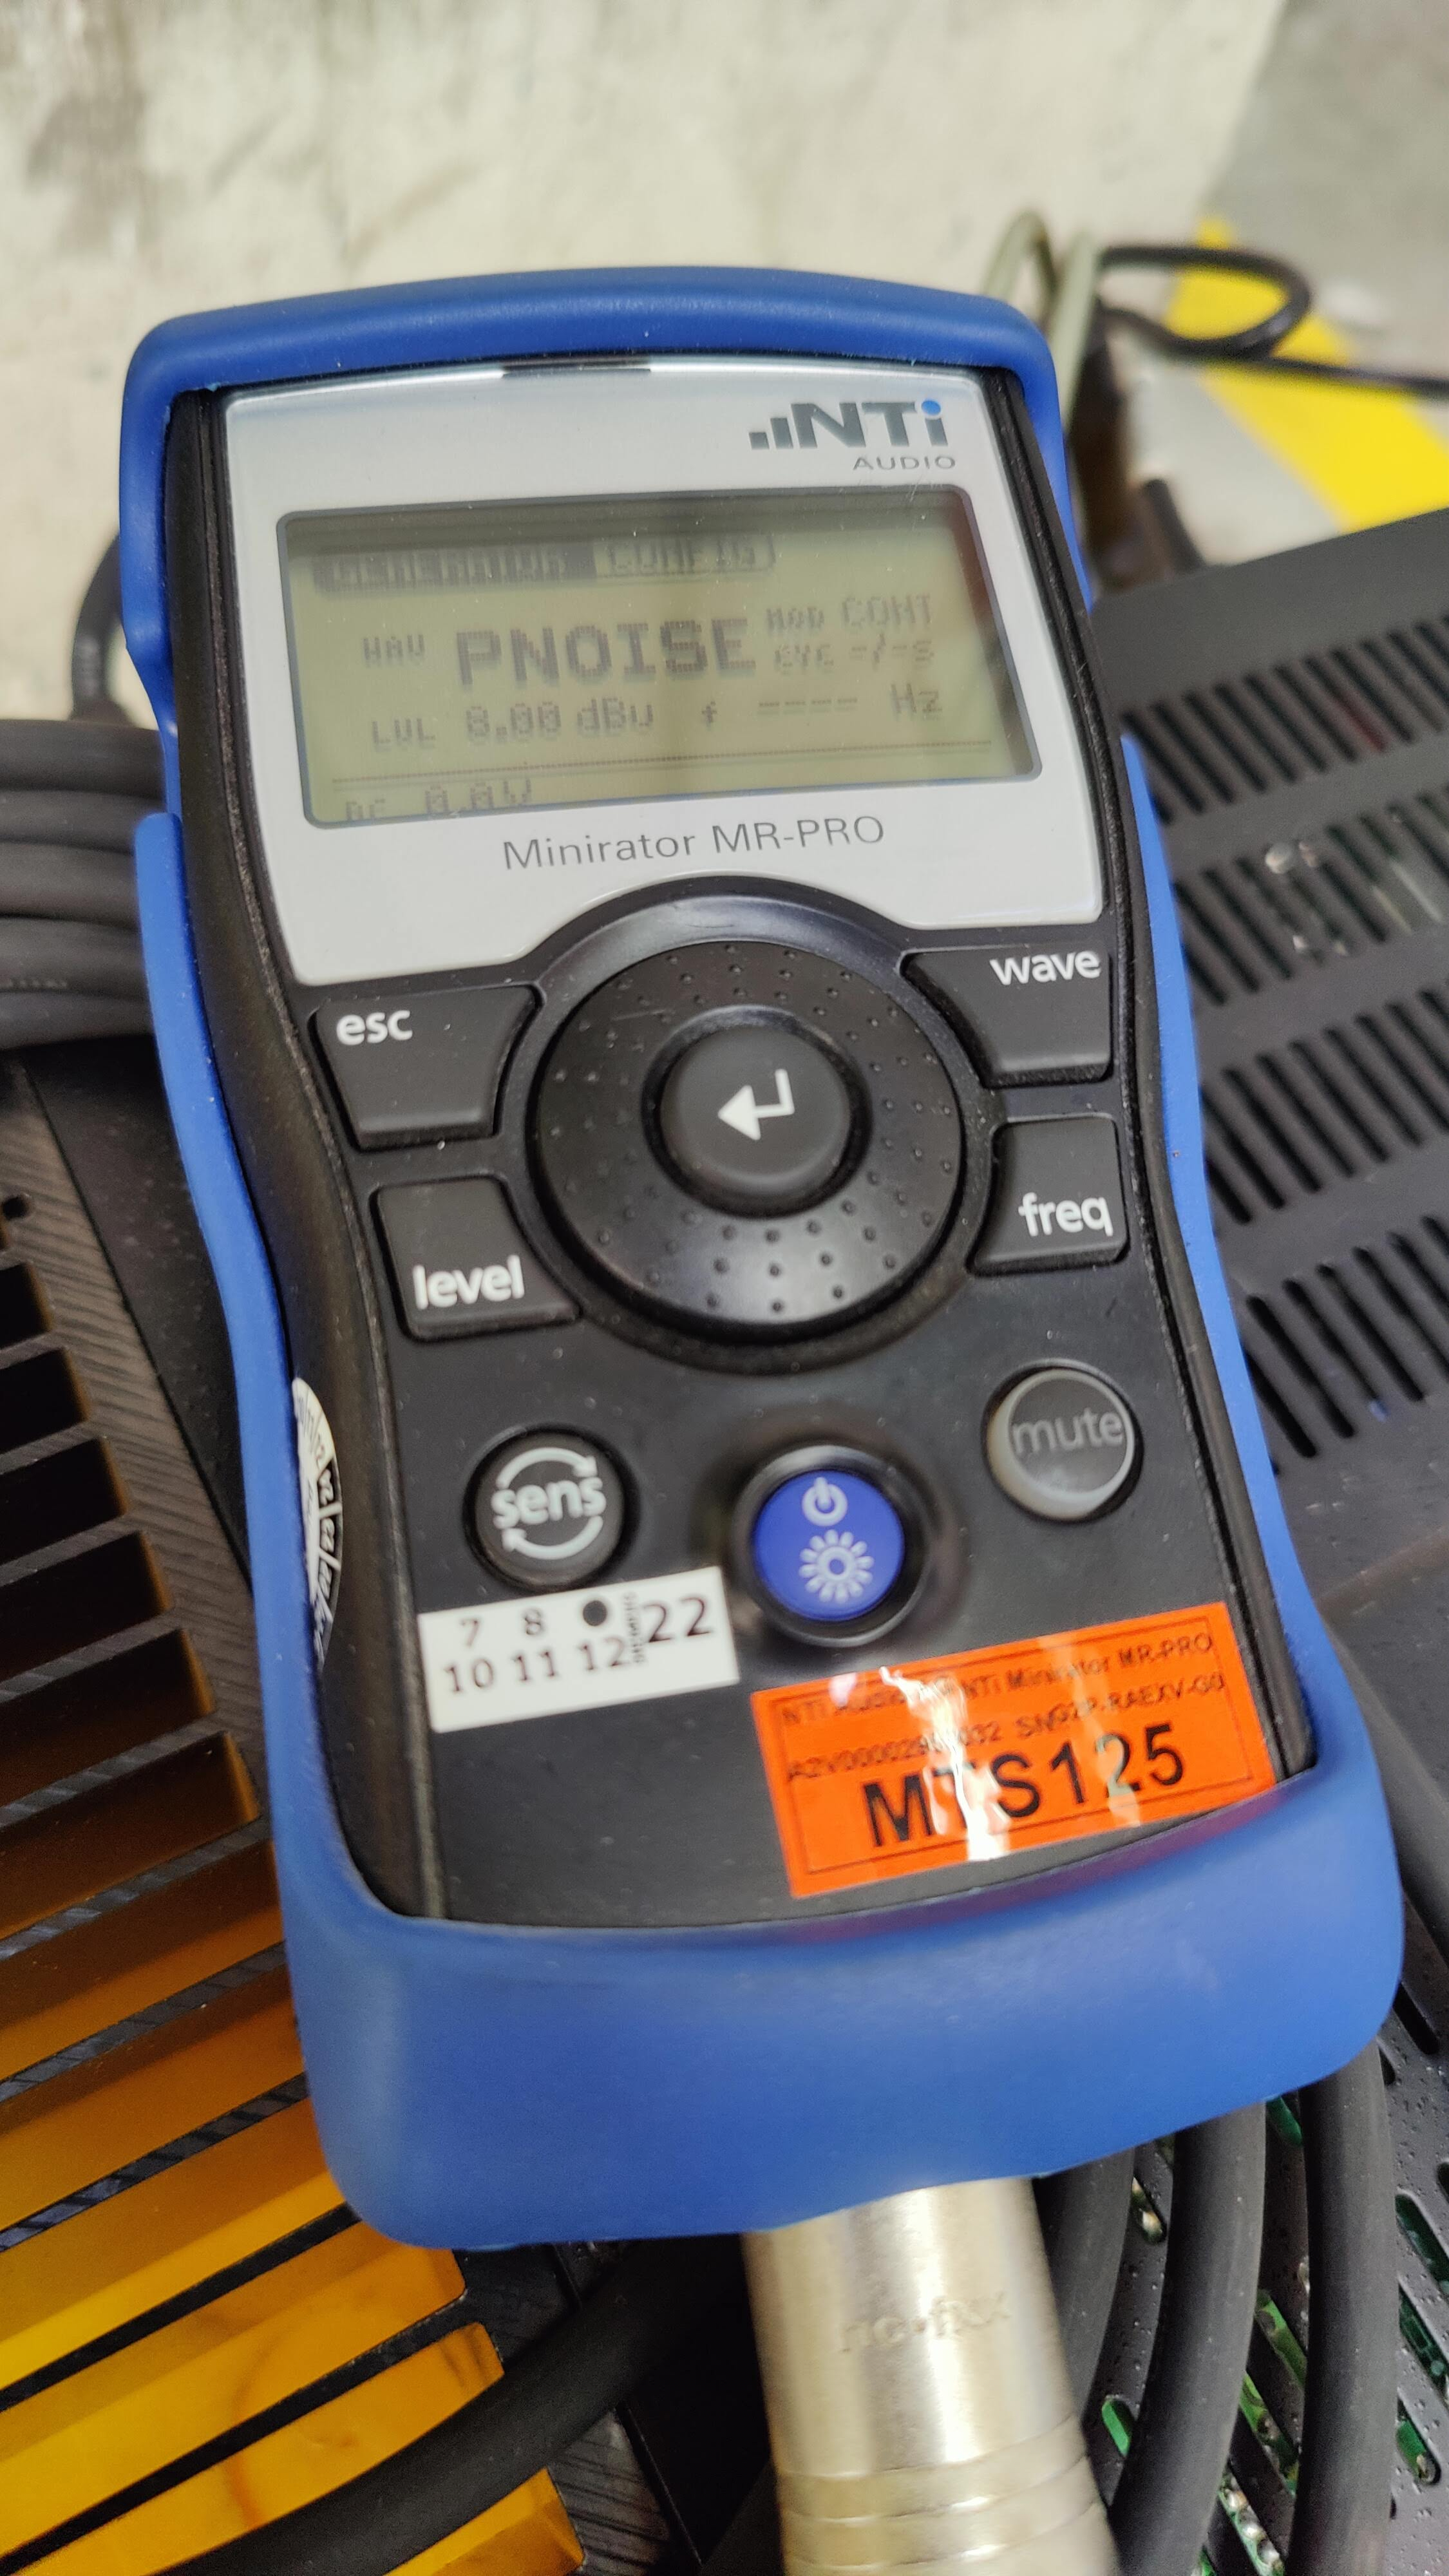
\includegraphics[width=\textwidth]{fig/signal_generator.jpg}
         \caption{NTI Minirator MR-PRO}
     \end{subfigure}
        \caption{Signal generator and amplifier}
        \label{fig:signalgenerator}
\end{figure}

\begin{figure}[H]
\begin{center}
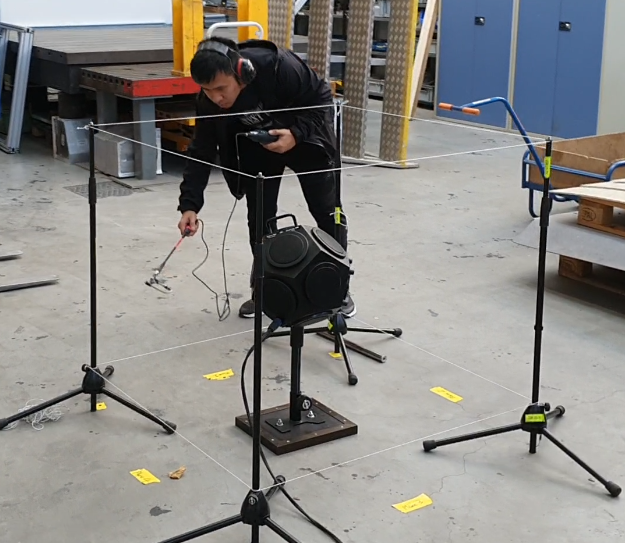
\includegraphics[width=12cm]{fig/Sound_power_measurement_2.png}
\caption{Scan method according to ISO 9614-2 \cite{din19969614}}
\label{fig:scanningmethod}
\end{center}
\end{figure}

\subsection*{Measurement results}

The measurment is post-processed using the Brüel \& Kjaer type 2270 hand-held analyzer and the result is shown in one-third octave band spectra. Fig. \ref{fig:SWL} shows the measured nonweighted (Z-weighting) sound power level (SWL ref $1e-12$ W) form 100 Hz to 2000 Hz. The measurement is carried out twice, the deviation of both measurements is within 0.3 dB in total power. For the finite element simulation, the averaged value of both measurments as show in fig. \ref{fig:average_SWL} will be used.

\begin{figure}[H]
     \centering
     \begin{subfigure}[b]{0.9\textwidth}
         \centering
         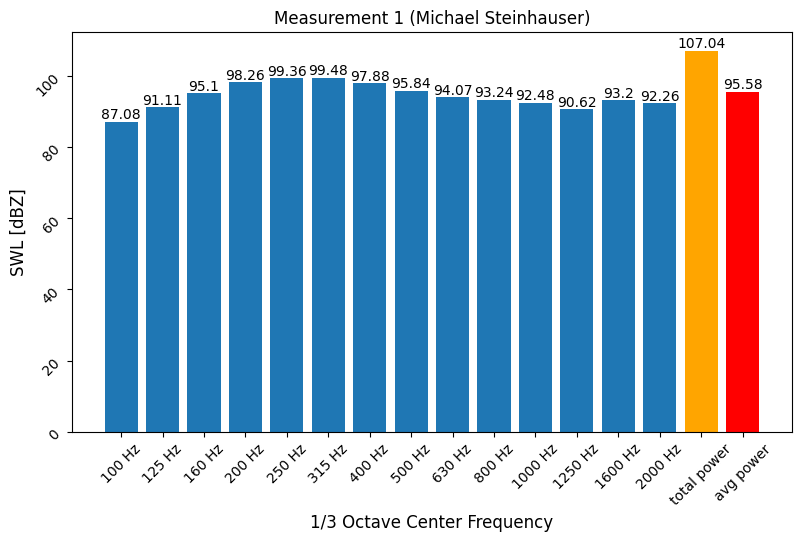
\includegraphics[width=\linewidth]{fig/SWL_1.png}
         \caption{Measurement series 1}
     \end{subfigure}
     \par\bigskip
     %\hspace{0.1\textwidth}
     %\hfill
     \begin{subfigure}[b]{0.9\textwidth}
         \centering
         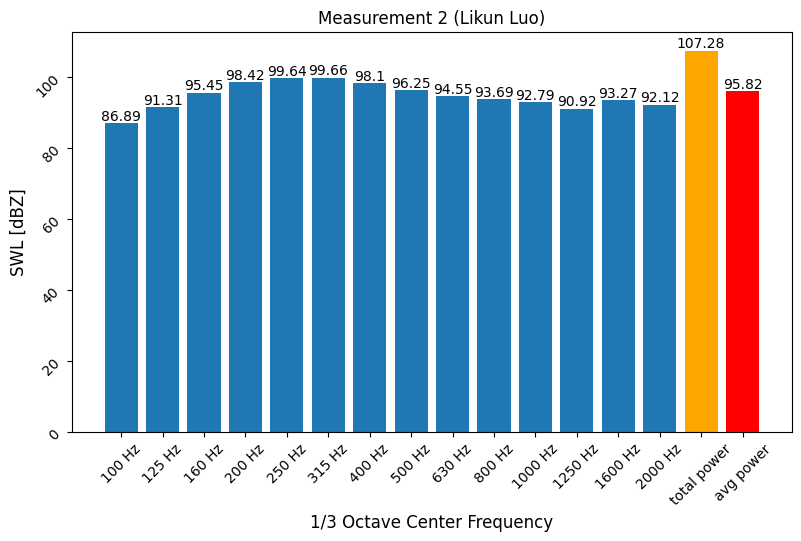
\includegraphics[width=\linewidth]{fig/SWL_2.png}
         \caption{Measurement series 2}
     \end{subfigure}
\end{figure}

\begin{figure}[H]\ContinuedFloat
     \centering
     \begin{subfigure}[b]{0.9\textwidth}
         \centering
         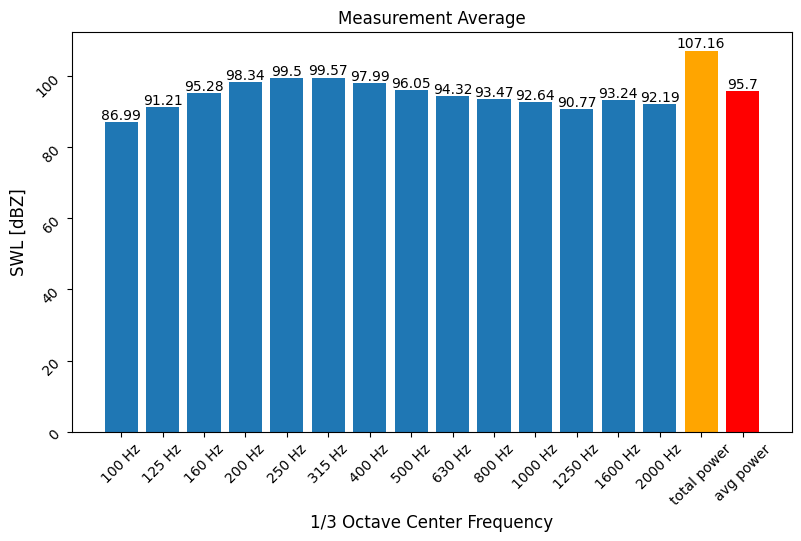
\includegraphics[width=\linewidth]{fig/SWL_average.png}
         \caption{Averaged value of both measurement series}
         \label{fig:average_SWL}
     \end{subfigure}
     
        \caption{Sound power spectra in 1/3-Octave band}
        \label{fig:SWL}
\end{figure}


\section{Pressure field measurement on a standing metro train}

In this section, the sound pressure measurement on a standing UBX metro with controlled excitation has been carried out. The aim to perform measurements under standstill condition is to avoid the uncertainties introduced by the complex real sources (e.g. wheel-rail interaction) in dynamic conditions. In such wise, the quality of the finite element model can be better assessed.

\subsection*{Measurement setup}

The measurement was performed on October 4, 2022 at company premises of Siemens Mobility Austria in 1110 Vienna. The measurement setup is shown in fig. \ref{fig:outersetup}. Fig. \ref{fig:ubxfrontview} shows the front car of the measurement vehicle of type Siemens U-Bahn Wien X. In order to approximate free field conditions as closely as possible, the measurement vehicle is parked in a relatively empty area of company premises avoiding environmental reflections as much as possible.

To evaluate the outer pressure field close to the carbody, 10 pressure microphones are arranged in a line array order, allowing simultaneous measurement along the height direction. As shown in fig. \ref{fig:ubxsideview}, the microphones are attached on a tripod at a distance of half meter to each other, the position of the microphones starts at 0.5 m and ends at 5 m above ground.

The acoustic excitation comes from an omnidirectional loudspeaker with pink noise as input signal, using the identical settings as in the previous acoustic power measurement. The loudspeaker is placed beneath the car underframe in the empty space between the bogie axle and the wheel axle, at about 55 cm above ground (Fig .\ref{fig:loudspeakerposition}). Measurements have been performed with 2 different loudspeaker locations. One at the front of bogie (Position A), and the other at the rear (Position B), as marked in fig. \ref{fig:ubxsideview}. The aim is to evaluate the possible asymetric effect caused by the anti-symmetric layout of the bogie components (e.g. brake discs), also it provides a validation for the latter finite element model, which will exploit the symmetry using image-source technique.

Due to the limited availability of the measurement vehicle, the measurement is concentrated on only one side of the vehicle, near the front bogie. In fig. \ref{fig:microphoneposition}, all measurement positions of the microphone array are shown and labeled. Position a is the starting position of measurement, it lies on the centerline of the bogie frame, 10 cm away from the carbody edge (Fig. \ref{fig:position_a}). The full description of measurement positions is found in the table below:

\begin{table}[H]
\begin{tabular}{|c|c|}
\hline
Position Label & Description                                                                     \\ \hline
a              & on bogie centerline , 10 cm away from carbody edge                              \\ \hline
b              & 50 cm out of bogie centerline in front direction, 10 cm away from carbody edge  \\ \hline
c              & 100 cm out of bogie centerline in front direction, 10 cm away from carbody edge \\ \hline
d              & 50 cm out of bogie centerline in rear direction, 10 cm away from carbody edge   \\ \hline
e              & 100 cm out of bogie centerline in rear direction, 10 cm away from carbody edge  \\ \hline
f              & on bogie centerline , 50 cm away from carbody edge                              \\ \hline
g              & on bogie centerline , 100 cm away from carbody edge                             \\ \hline
h              & on bogie centerline , 150 cm away from carbody edge                             \\ \hline
i              & on bogie centerline , 200 cm away from carbody edge                             \\ \hline
\end{tabular}
\caption{Description of measurement positions}
\label{tab:measurement_positons}
\end{table}

At each measurement position, the multi-channel time-varing signal of the pressure field is captured by the Müller-BBM PAK MKII data acquisition system. The duration of single measurement run is set to 15 seconds. The captured time signal will be post-processed using the provided Müller-BBM PAK software suit.

\begin{figure}[H]
     \centering
     \begin{subfigure}[b]{0.7\textwidth}
         \centering
         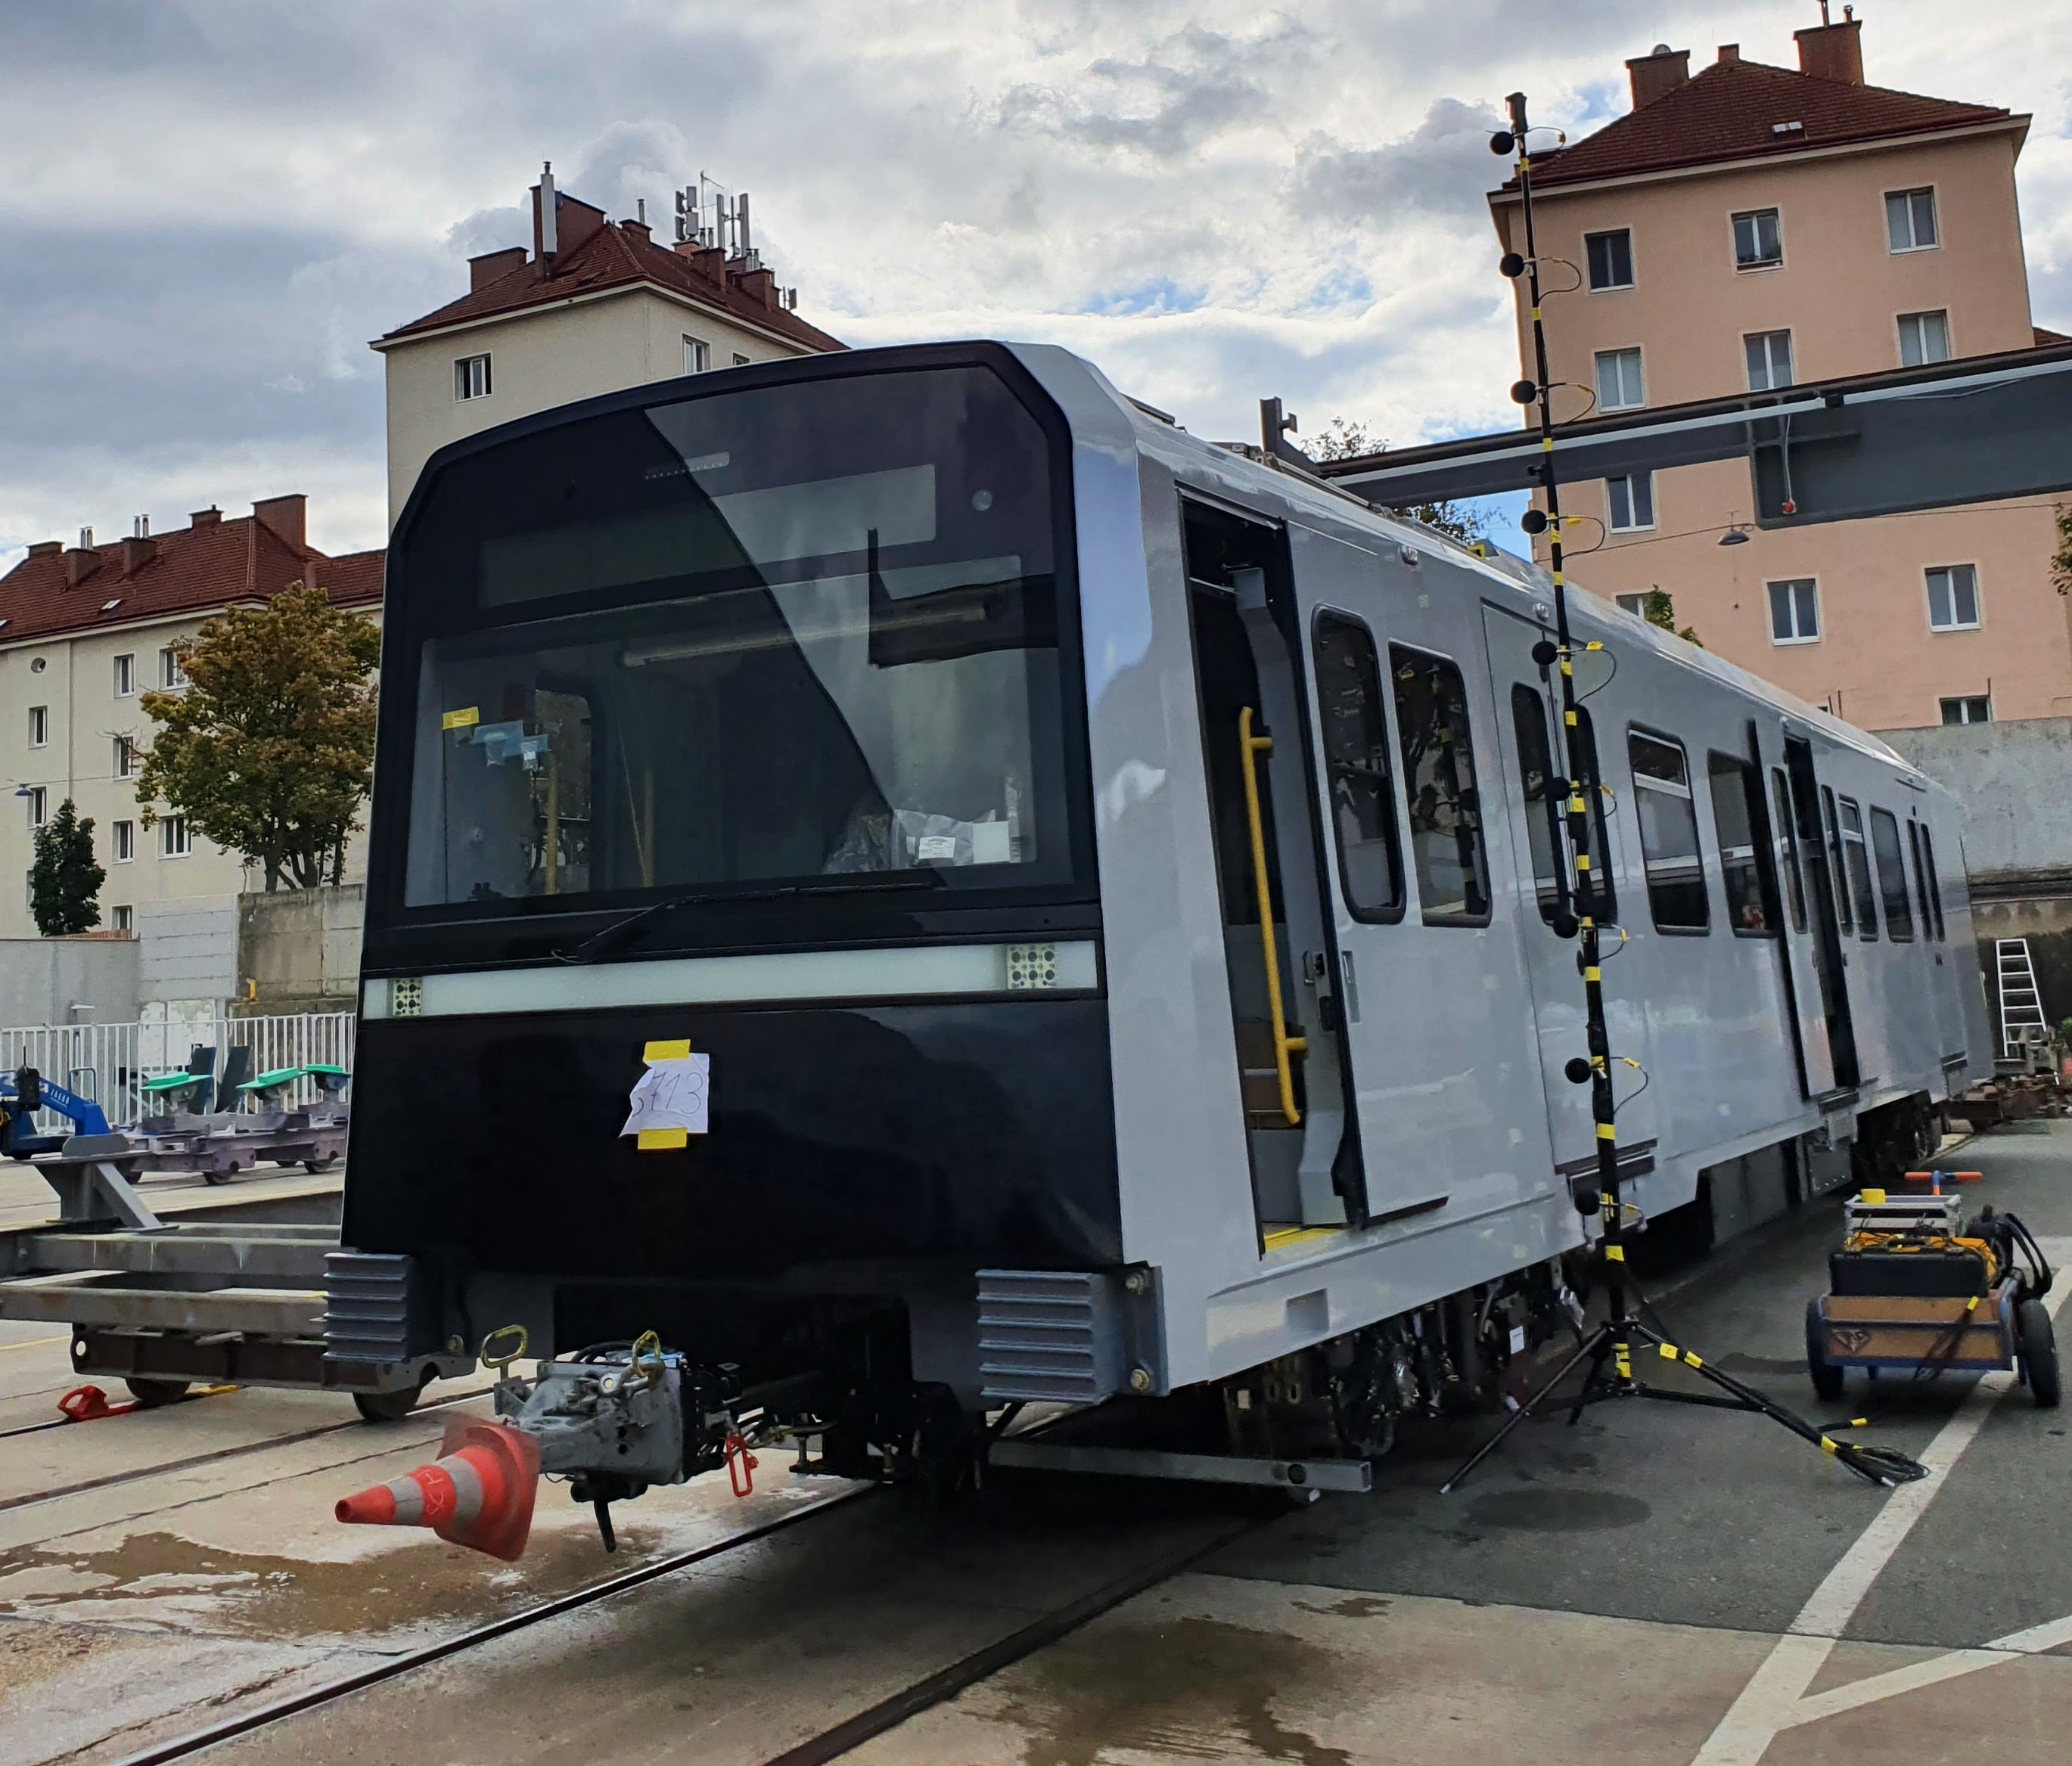
\includegraphics[width=\linewidth]{fig/Static_measurement_front_view.jpg}
         \caption{Front view}
         \label{fig:ubxfrontview}
     \end{subfigure}
     %\par\bigskip
     %\hspace{0.1\textwidth}
     %\hfill
\end{figure}

\begin{figure}[H]\ContinuedFloat
    \centering
    \begin{subfigure}[b]{\textwidth}
         \centering
         \includegraphics[width=\linewidth]{fig/Static_measurement_side_view.png}
         \caption{Side view}
         \label{fig:ubxsideview}
     \end{subfigure}
     \caption{Outer pressure field measurement setup}
     \label{fig:outersetup}
\end{figure}

\begin{figure}[H]
     \centering
     \begin{subfigure}[b]{0.4\textwidth}
         \centering
         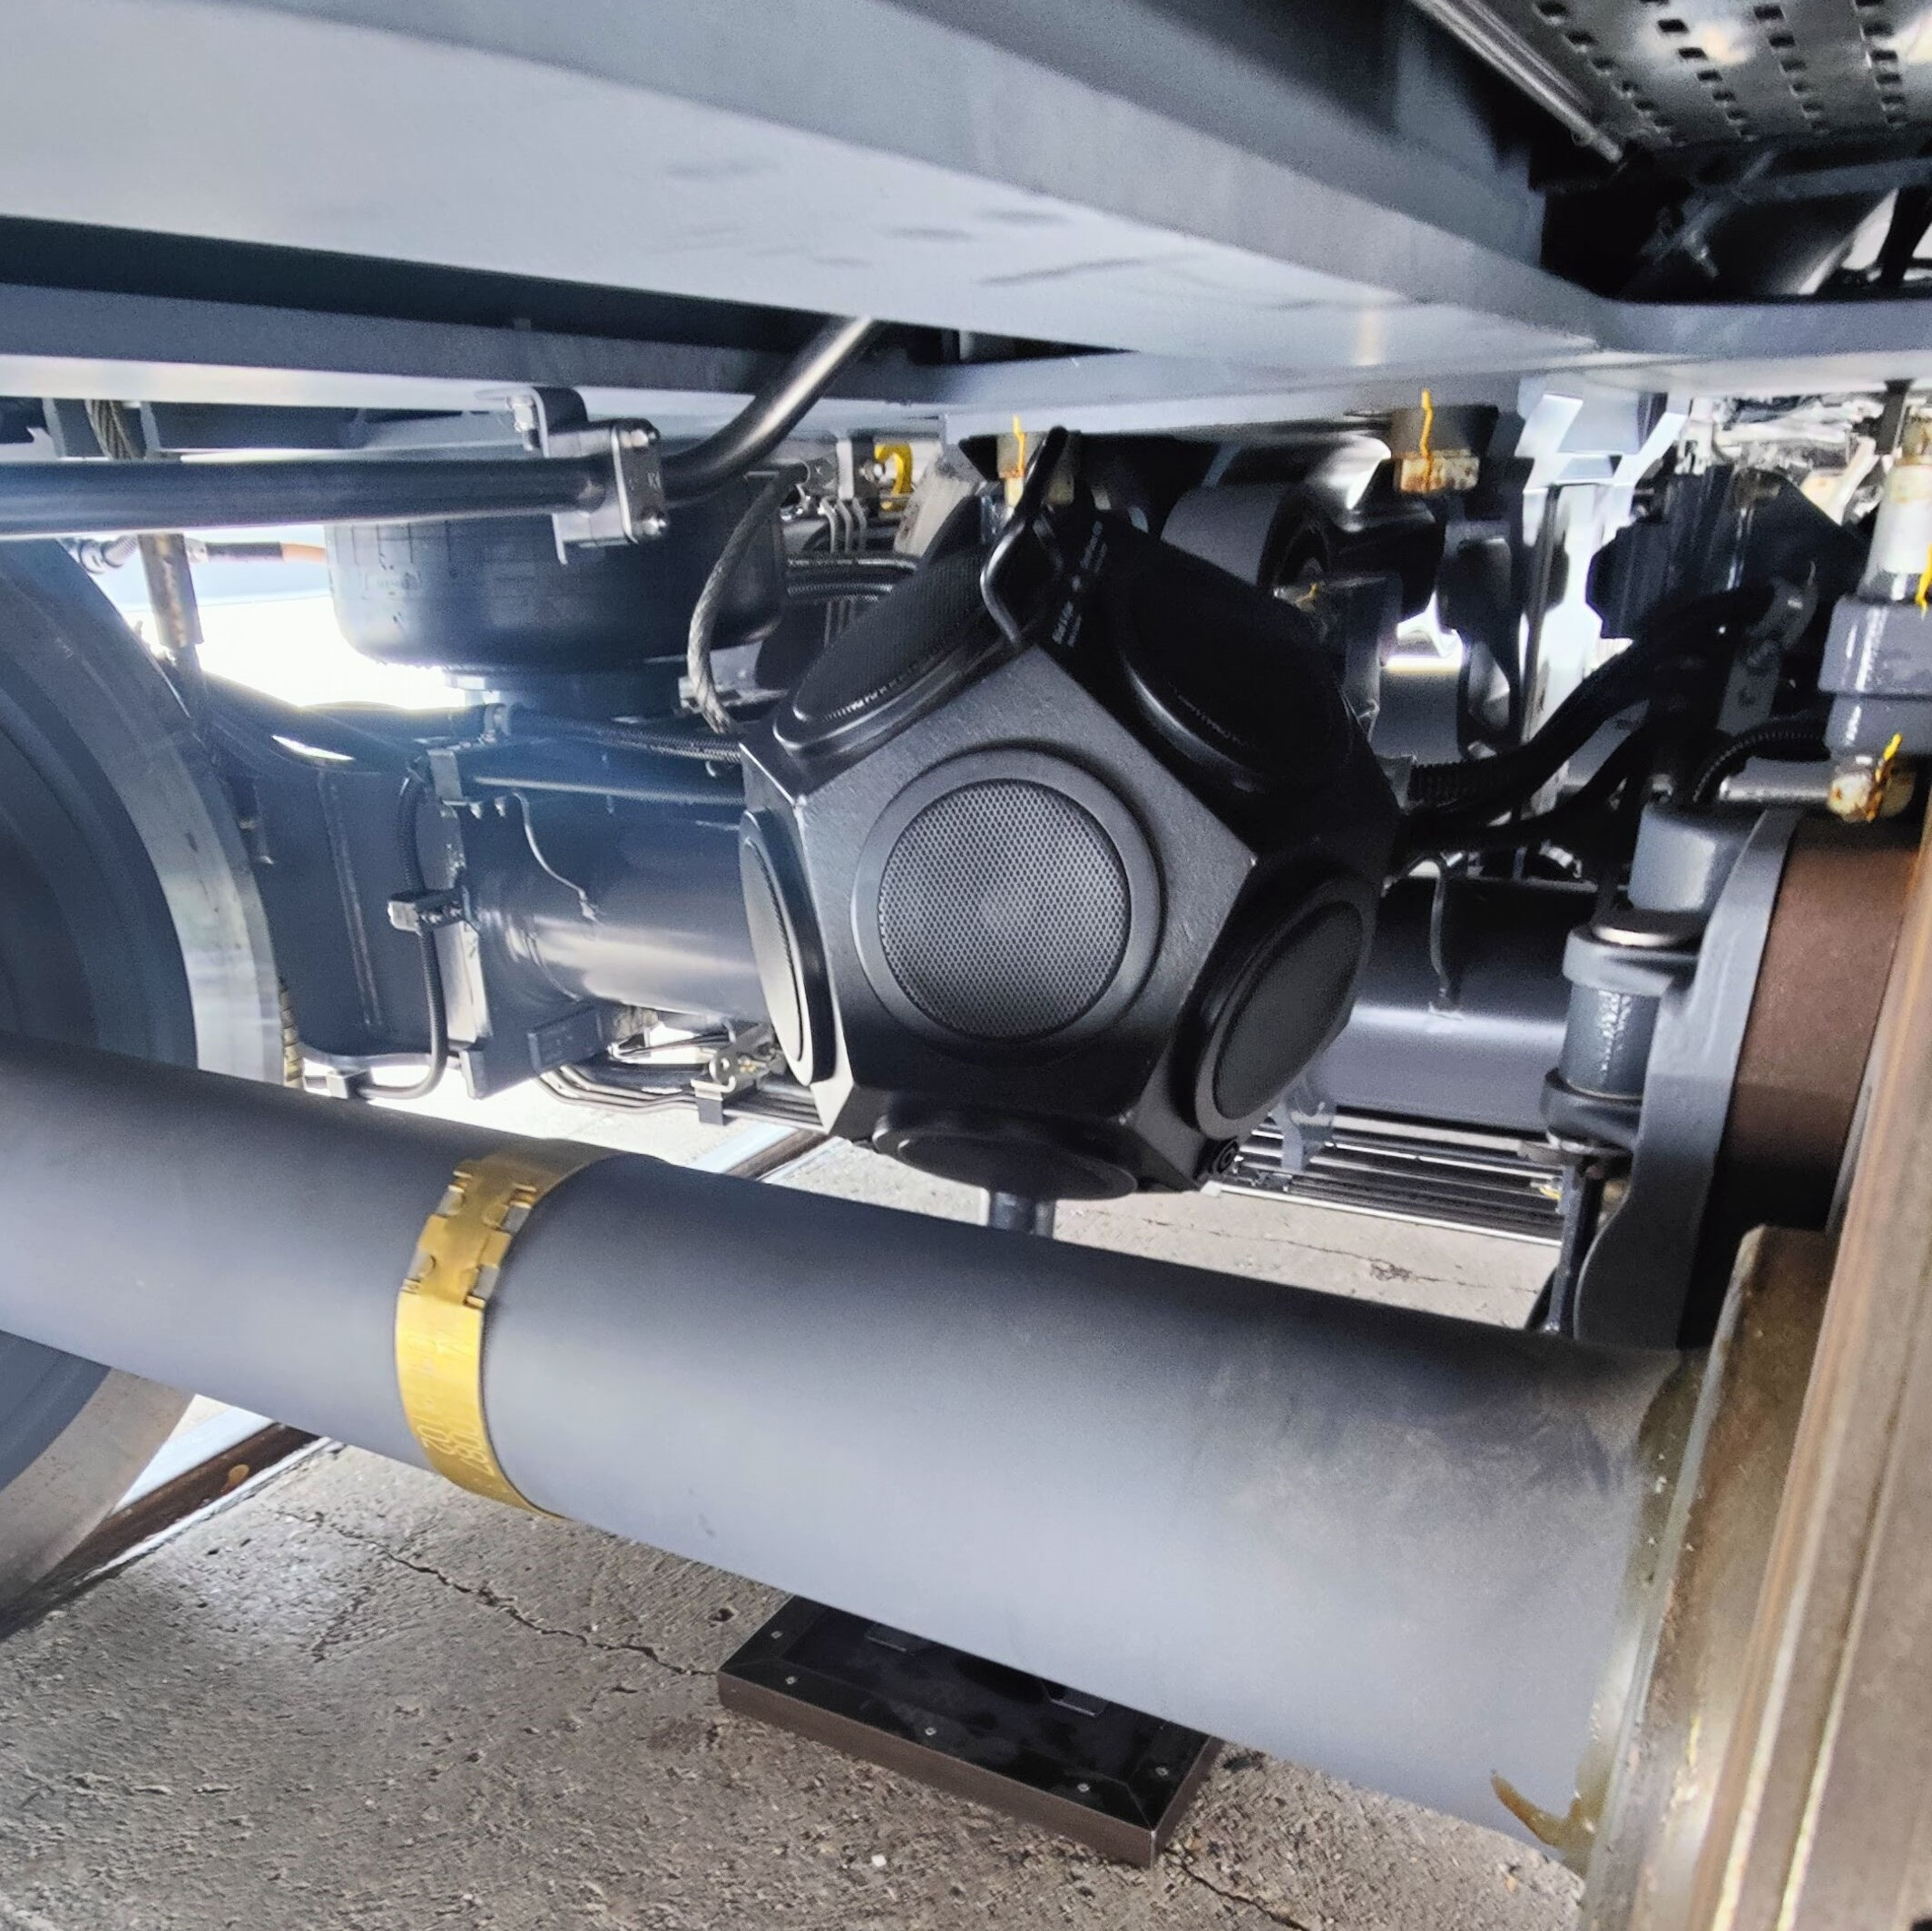
\includegraphics[width=\linewidth]{fig/loudspeaker_position_A.jpg}
         \caption{Position A: front of bogie}
     \end{subfigure}
     %\par\bigskip
     \hspace{0.1\textwidth}
     %\hfill
     \begin{subfigure}[b]{0.4\textwidth}
         \centering
         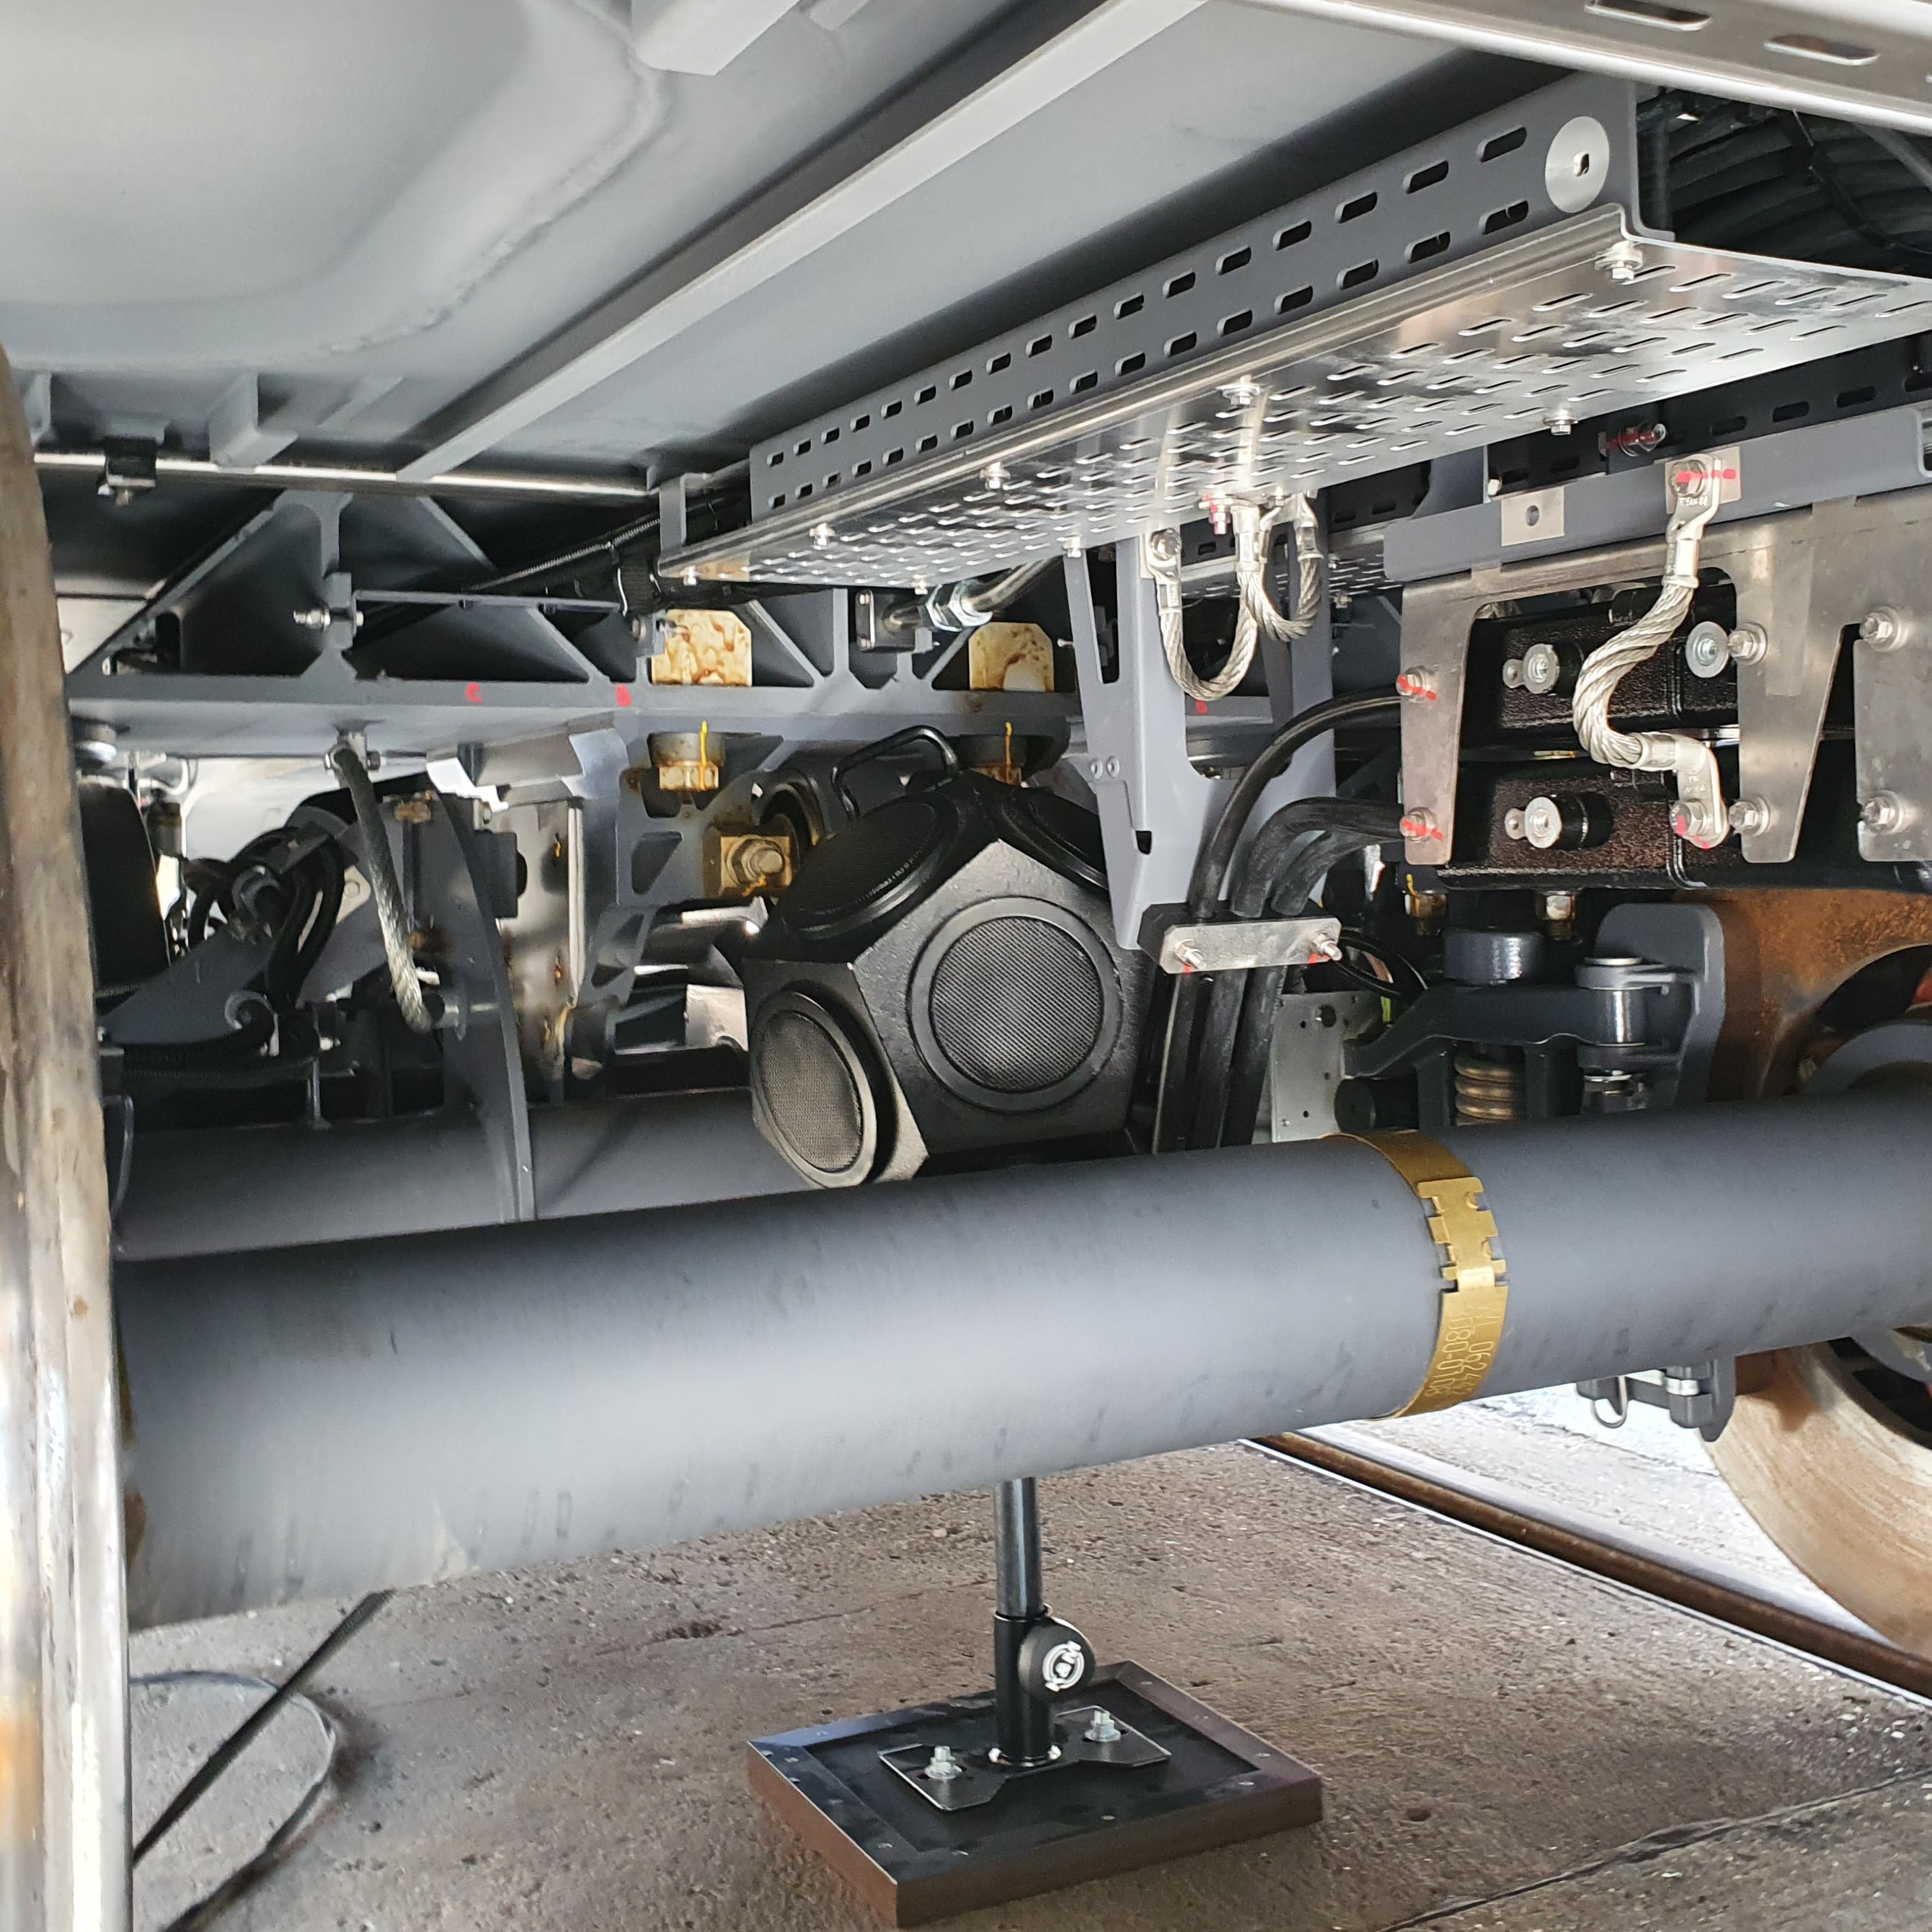
\includegraphics[width=\linewidth]{fig/loudspeaker_position_B.jpg}
         \caption{Postition B: rear of bogie}
     \end{subfigure}
     \caption{Loudspeaker locations}
     \label{fig:loudspeakerposition}
\end{figure}

\begin{figure}[H]
     \centering
     \begin{subfigure}[b]{\textwidth}
         \centering
         \includegraphics[width=\linewidth]{fig/Measurement_positions.png}
         \caption{Measurement positions a to i}
     \end{subfigure}
     %\par\bigskip
     %\hspace{0.1\textwidth}
     %\hfill
\end{figure}

\begin{figure}[H]\ContinuedFloat
    \centering
    \begin{subfigure}[b]{0.6\textwidth}
         \centering
         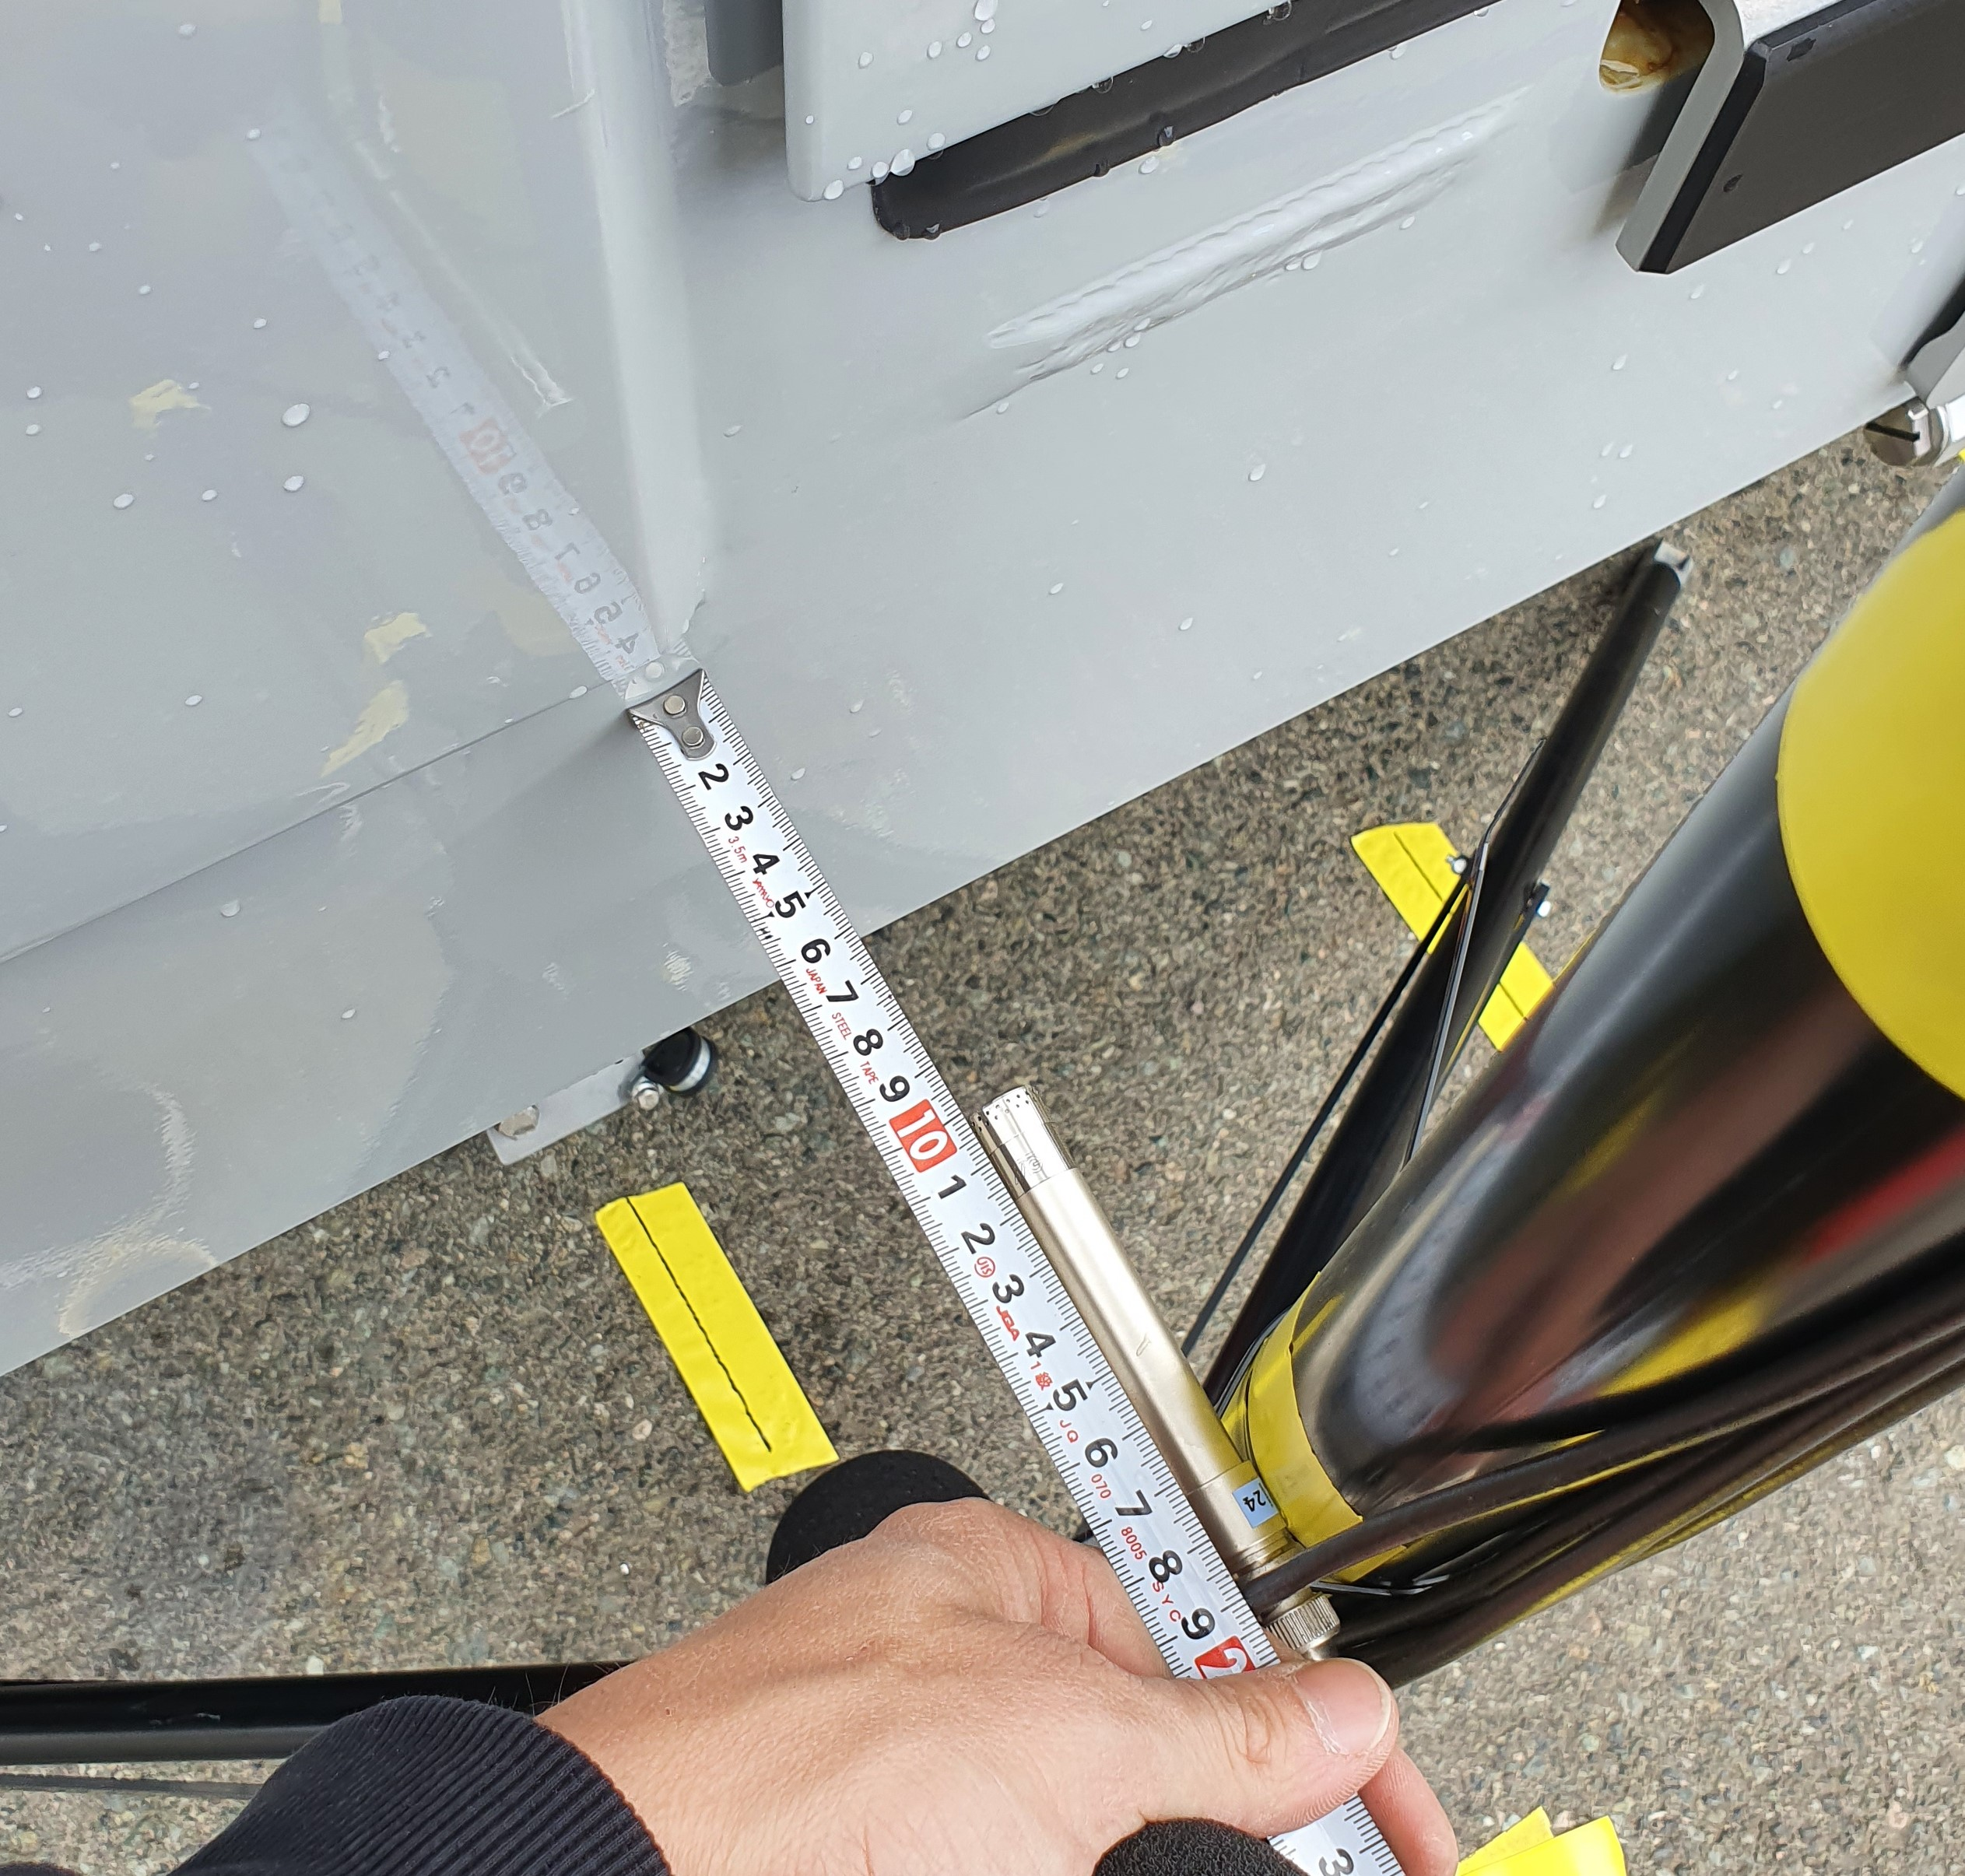
\includegraphics[width=\linewidth]{fig/position_of_microphones.jpg}
         \caption{Postition a: centerline of the bogie, 10 cm away from carbody edge}
         \label{fig:position_a}
     \end{subfigure}
     \caption{Measurement positions of microphone array}
     \label{fig:microphoneposition}
\end{figure}

\subsection*{Measurement results}

In fig. \ref{fig:timedomain}, the measured time signal of microphone 1 (0.5 m above ground) at measurment position a (front bogie centerline, 10 cm away from carbody) with loudspeaker placed at the front of bogie can be seen. The signal is converted into frequency domain using fourier transformation as shown in fig. \ref{fig:frequencydomain}. The post-processing can be done directly in the provided software suit Müller-BBM PAK 6.x, fig. \ref{fig:fftparameter} shows a screenshot of the GUI and the FFT parameter used is circled.

In fig. \ref{fig:frequencydomain}, the blue curve shows the amplitude of acoustic pressure in narrow band resolution. The narrow band data is converted to 1/n octave form by summing up the amplitude of narrow-band spectral lines contained within the corresponding frequency bandwidth. The advantage of post-processing the data into octave bands is that it provides clearer information about the frequency composition of the noise signal. For example, it can be observed that in the 1/3 octave curve in fig. \ref{fig:frequencydomain}, the peak of the SPL appears at 315 Hz, which also matches the peak in the SWL spectrum of the sound source as shown in fig. \ref{fig:average_SWL}.

\begin{figure}[H]
    \centering
    \begin{subfigure}[b]{0.6\textwidth}
        \centering
        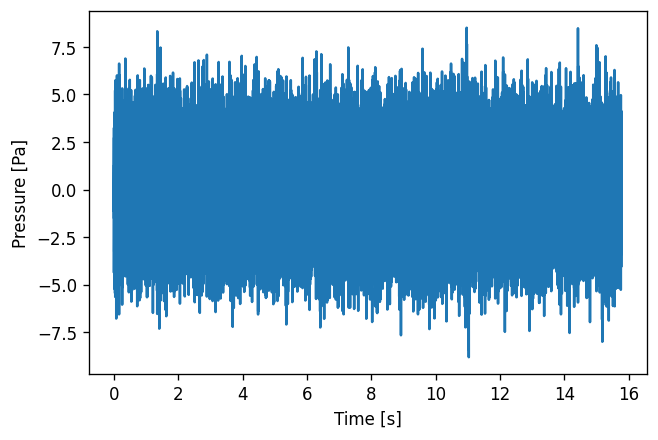
\includegraphics[width=\linewidth]{fig/time_signal.png}
        \caption{Time domain}
        \label{fig:timedomain}
    \end{subfigure}

    \begin{subfigure}[b]{0.6\textwidth}
        \centering
        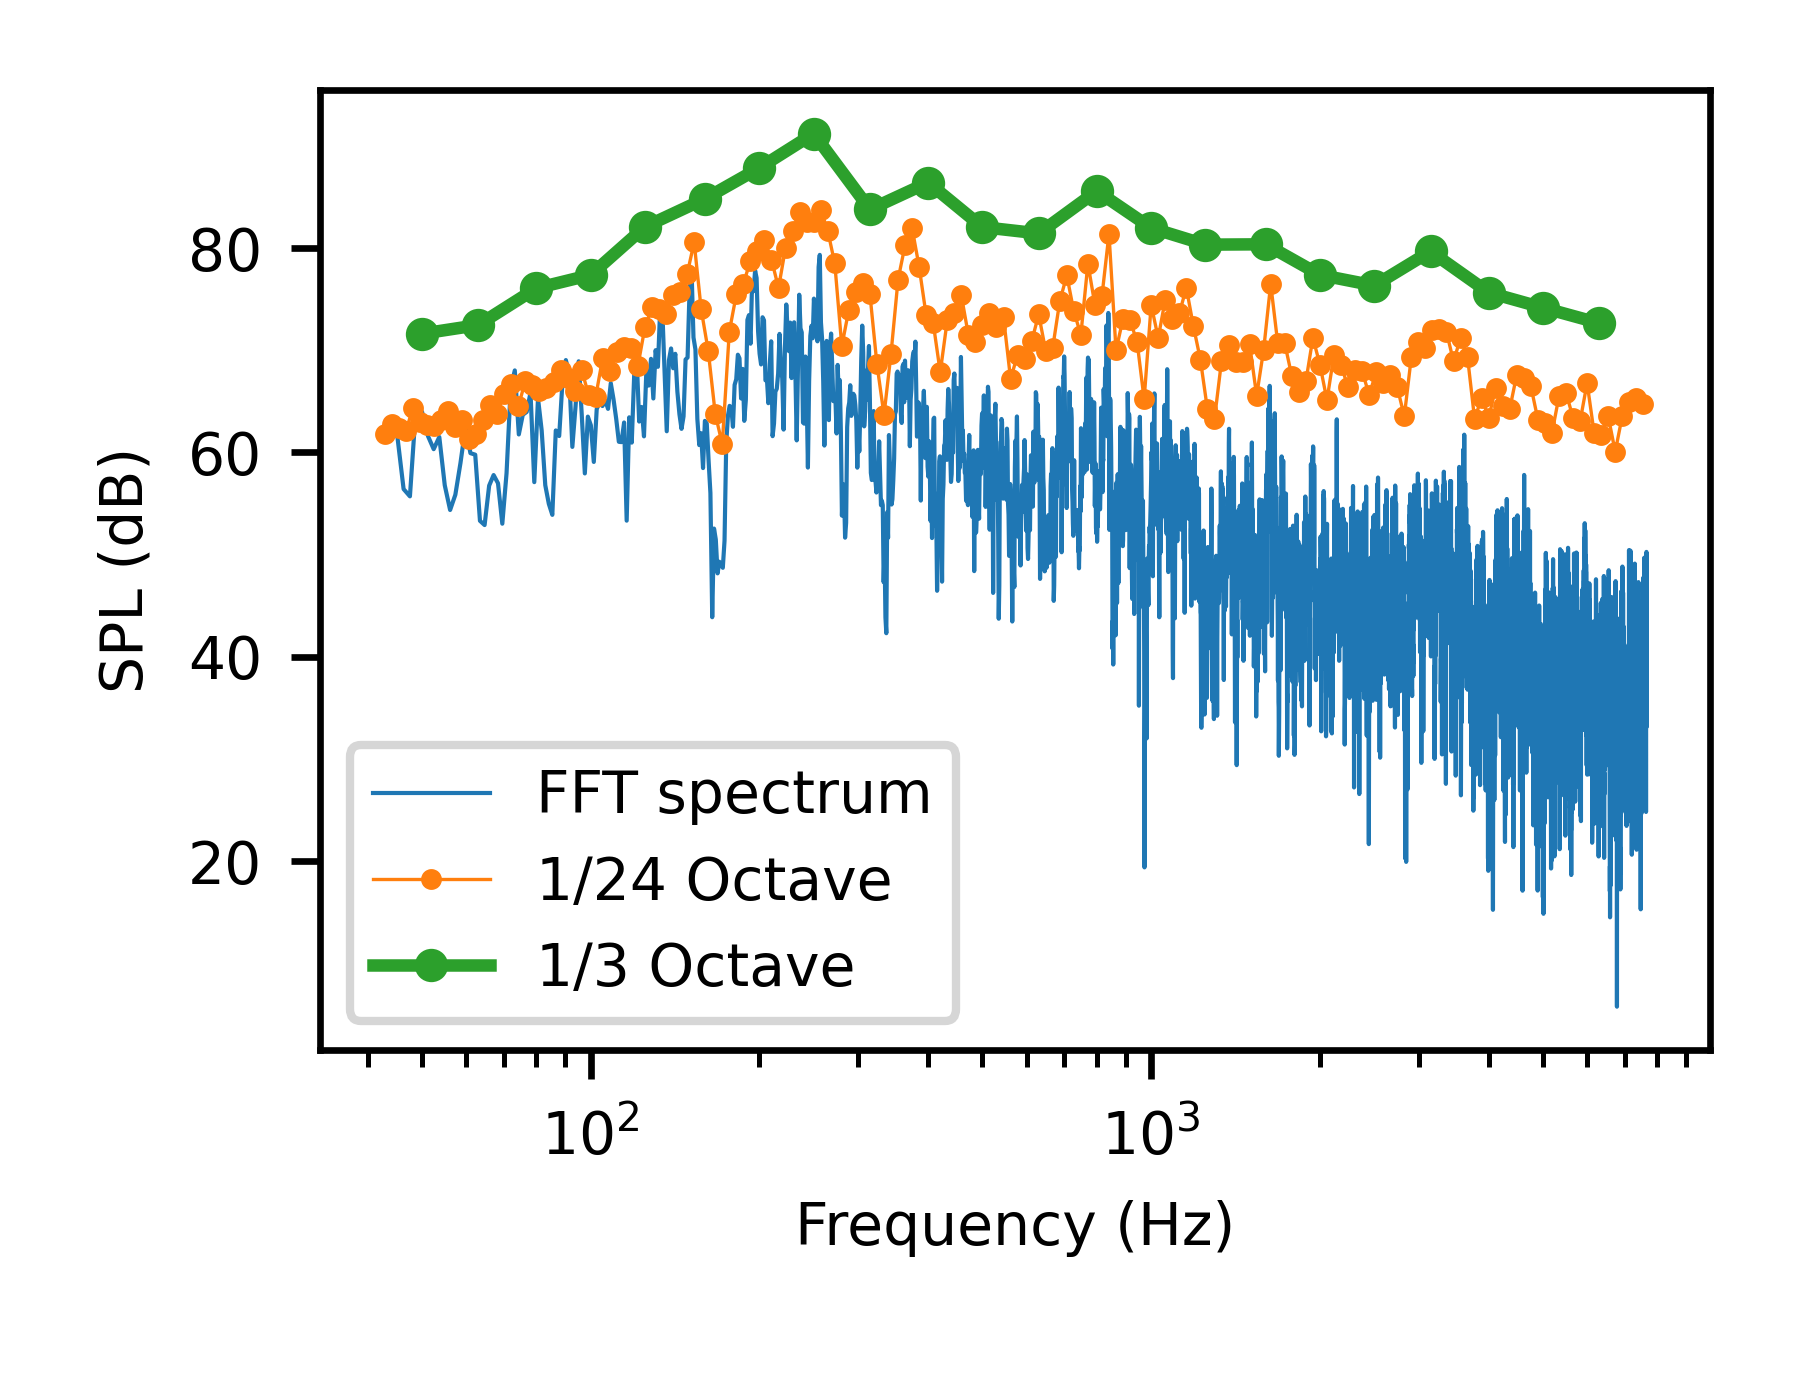
\includegraphics[width=\linewidth]{fig/fft_spectra.png}
        \caption{Frequency domain}
        \label{fig:frequencydomain}
    \end{subfigure}
    
    \caption{Mesurement data at position a, microphone 1 (0.5 m), loudspeaker front}
    \label{fig:measurementsignal}
\end{figure}

\begin{figure}[H]
    \centering
    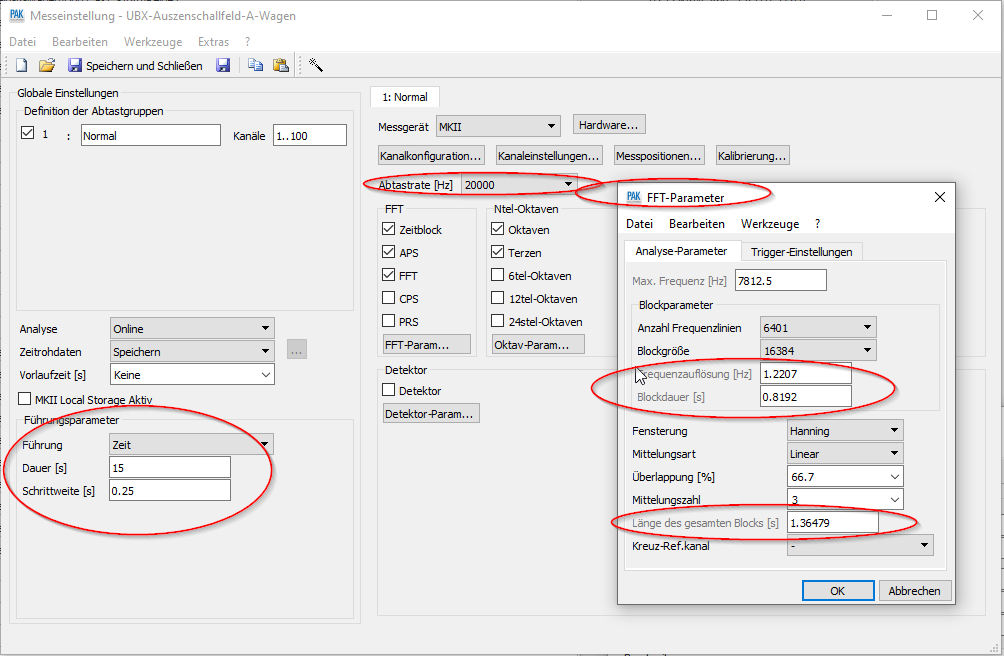
\includegraphics[width=\linewidth]{fig/fft_parameter.png}
    \caption{FFT parameter used}
    \label{fig:fftparameter}
\end{figure}

\begin{figure}[H]
    \centering
     \begin{subfigure}[b]{0.49\textwidth}
        \centering
        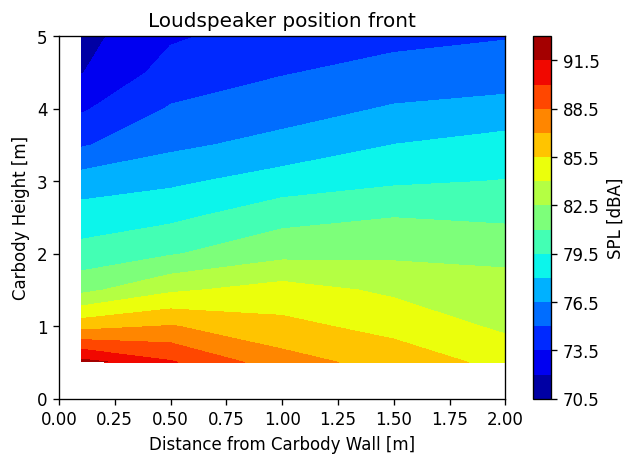
\includegraphics[width=\textwidth]{fig/pressure_field_loudspeaker_front.png}
        \caption{Loudspeaker position front}
    \end{subfigure}
    \begin{subfigure}[b]{0.49\textwidth}
        \centering
        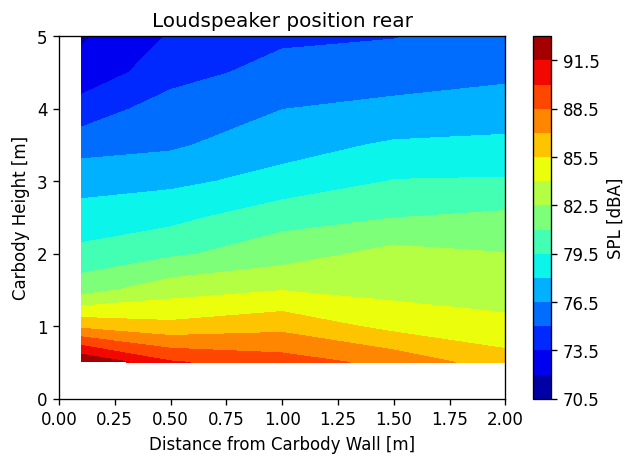
\includegraphics[width=\textwidth]{fig/pressure_field_loudspeaker_rear.png}
        \caption{Loudspeaker position rear}
    \end{subfigure}
        \caption{Pressure field around carbody}
        \label{fig:pressurefield}
\end{figure}

In fig. \ref{fig:pressurefield}, a visualization of the total pressure field around the carbody is shown. The horizontal axis represents the distance from carbody wall, the vertical axis the height above ground and the color the a-weighted total pressure level, respectively.  The white space in the plot is due to the missing data in the measurement since the measurment positions start at 10 cm away from carbody wall and half meter above ground. Comparing the pressure field of the two different loudspeaker locations, the asymmetric effect introduced by the brake disc can be observed. The brake disc of the front wheel axle standing in the transmisson path of the loudspeaker seems to block a part of the acoustic wave.

\begin{figure}[H]
    \centering
     \begin{subfigure}[b]{0.6\textwidth}
        \centering
        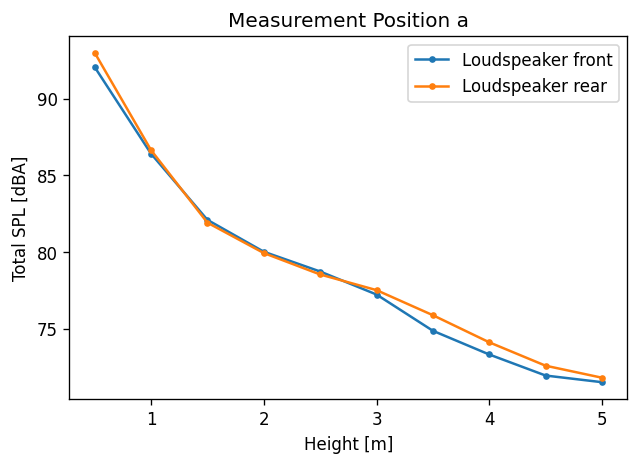
\includegraphics[width=\linewidth]{fig/pressure_over_height_pos_a.png}
        \caption{Measurement position a}
        \label{fig:SPLoverheight_pos_a}
    \end{subfigure}

    \begin{subfigure}[b]{0.6\textwidth}
        \centering
        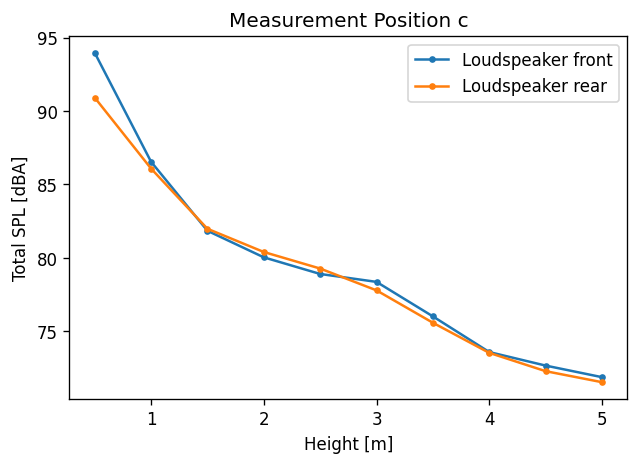
\includegraphics[width=\linewidth]{fig/pressure_over_height_pos_c.png}
        \caption{Measurement position c}
        %\label{fig:frequencydomain}
    \end{subfigure}
    \caption{Total SPL as a function of the height above ground}
    \label{fig:SPLoverheight}
\end{figure}

In order to compare the pressure field quantitatively, one can plot the acoustic pressure as function of height for different measurement positions, which can be seen in the figures above. In \ref{fig:SPLoverheight_pos_a} it can be observed that at measurement position a, the pressure curve caused by loudspeaker at different locations shares similar shape, and the pressure is strictly decreasing over carbody height.

\begin{figure}[H]
    \centering
     \begin{subfigure}[b]{0.6\textwidth}
        \centering
        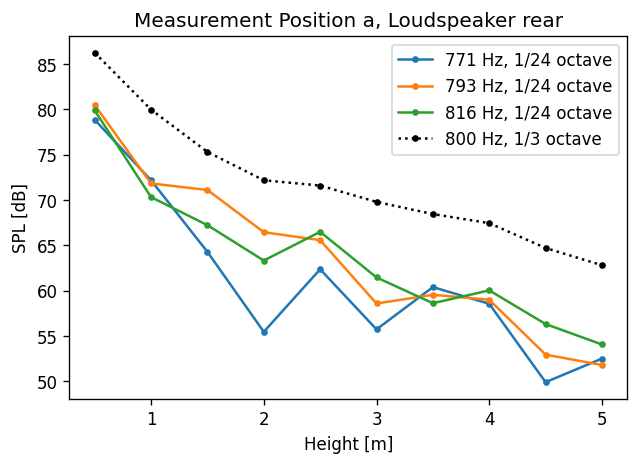
\includegraphics[width=\linewidth]{fig/pressure_over_height_800Hz.png}
        \caption{800 Hz}
        \label{fig:SPLoverheight_frequency_800Hz}
    \end{subfigure}

    \begin{subfigure}[b]{0.6\textwidth}
        \centering
        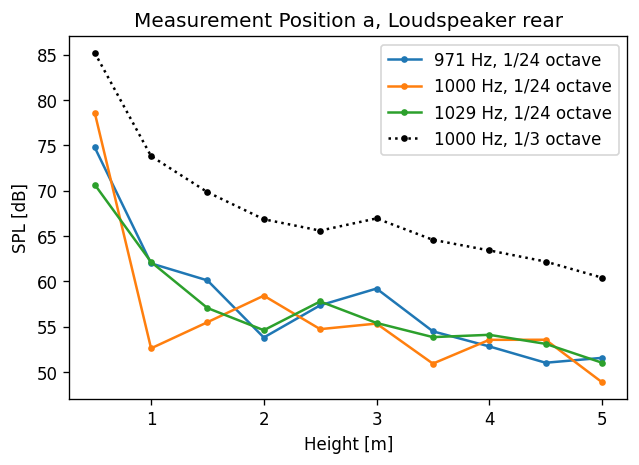
\includegraphics[width=\linewidth]{fig/pressure_over_height_1000Hz.png}
        \caption{1000 Hz}
        \label{fig:SPLoverheight_frequency_1000Hz}
    \end{subfigure}
    \caption{SPL as a function of the height above ground, single-frequency, measurment position a, loudspeaker rear}
    \label{fig:SPLoverheight_frequency}
\end{figure}

In fig. \ref{fig:SPLoverheight_frequency}, the sound pressure level over height for different 1/n octave band center frequencies is displayed. In the 1/24 octave resolution, several local minima in the curve shape can be observed, e.g. for 771 Hz in fig. \ref{fig:SPLoverheight_frequency_800Hz} or for 1000 Hz in fig. \ref{fig:SPLoverheight_frequency_1000Hz}, which are caused by the destructive interference of the acoustic wave. The destructive interference can also be observed in the pressure field of the single frequency band as shown in fig. \ref{fig:pressurefield_1000Hz}, sinks in acoustic field are to be found at about 1 m and 3.5 m height, respectively, which correspond to the position of the local minima in fig. \ref{fig:SPLoverheight_frequency_1000Hz}.


\begin{figure}[H]
    \centering
    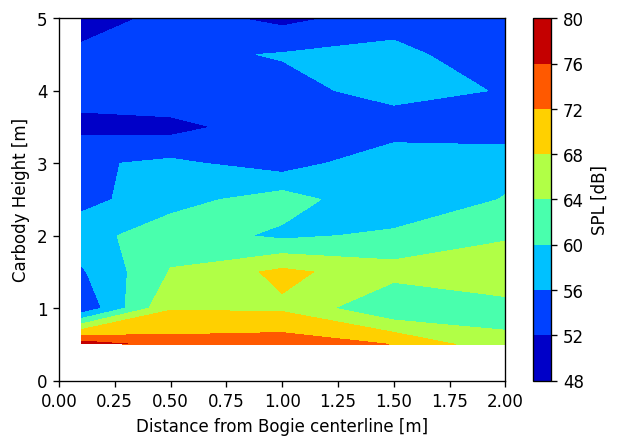
\includegraphics[width=0.6\linewidth]{fig/pressure_field_1000Hz.png}
    \caption{Pressure field of 1/24-octave frequency 1000 Hz, loudspeaker rear}
    \label{fig:pressurefield_1000Hz}
\end{figure}
